\documentclass[10pt,twocolumn]{confpaper}

%%%%%%%%%%%%%%%%%%%%  INCLUDES  %%%%%%%%%%%%%%%%%%%%%%%%%%
\usepackage{pifont}
\usepackage{algorithm}
\usepackage{algorithmic}
%%%%%%%%%%%%%%%%%%%%  LOCALS  %%%%%%%%%%%%%%%%%%%%%%%%%%%%

\newcommand{\system}{{OCDN}}
\def\checkmark{\tikz\fill[scale=0.4](0,.35) -- (.25,0) -- (1,.7) -- (.25,.15) -- cycle;}
\graphicspath{ {./figures/} }
\newcommand{\annie}[1]{\emph{\color{blue}(#1)}}


%%%%%%%%%%%%%%%%%%%%  TITLE/AUTHORS  %%%%%%%%%%%%%%%%%%%%%

\date{}
\title{\LARGE{\bf OCDN: Oblivious Content Distribution Networks}}
\author{
\aufnt{} \\
\affaddr{}
}

%%%%%%%%%%%%%%%%%%%%  START OF DOCUMENT  %%%%%%%%%%%%%%%%%

\begin{document}

\maketitle

%\AcmCopyright
%\ToAppear

\begin{sloppypar}




\subsection*{Abstract}

As the Internet continues to grow, it does so without national borders, 
raising the question of how data should be governed, by whom, and 
under what circumstances.  Different jurisdictions follow different policies 
and regulations, particularly on the topic of data privacy.  For example, the Safe
Harbor framework was developed to allow trans-Atlantic data flow while ensuring 
the privacy of European Union citizens' data.  Along with determining the invalidity 
of the framework, the courts are where most battles on data 
privacy have been fought while technology development with jurisdictional 
differences in mind has been left to the side. In this work, 
we focus on the privacy implications of cross-border data flows and data 
storage, and how technology can be designed to protect citizens' data, regardless 
of the jurisdiction in which the client, data, or service resides.  We highlight 
some of the historical court decisions, ongoing jurisdictional debates, and evaluate 
some of the proposed systems and techniques in terms of how well they provide data protection 
for either data at rest or data in motion.  Lastly, we explain and discuss how 
technology can play a role in designing systems to facilitate data privacy in 
the face of an overreaching government or conflicting jurisdictional policies.

\ifthenelse{\equal{\onlyAbstract}{no}}{% !onlyAbstract


\section{Introduction}
\label{sec:intro}

%Governments are increasingly using their authority to access data from
%their citizens and foreigners, even when this data may be stored overseas.  For
%example, in a
%recent case, the United States government tried to compel Microsoft to
%surrender data about U.S. citizens, even when the data itself was stored
%abroad~\cite{microsoft_ireland}. Users may also face the converse problem, where access to their data
%may depend on the laws of the country where their data is stored. Recent work,
%for example, highlights the possibility that governments may move data across
%borders to facilitate surveillance~\cite{arnbak2015loopholes}.  

As Content Delivery Networks (CDNs) host more content,
they are fast becoming targets of requests for information about their content
and who is requesting it, as well as requests for takedown of material. The shifting legal and political landscape suggests that CDNs may soon face liability for the content that they host. For example, the European Union has been considering laws that
would remove safe harbor protection on copyright infringement for online
service providers if they do not deploy tools that can automatically inspect
and remove infringing content~\cite{eu-copyright}. In the United States,
various laws under consideration threaten aspects of Section 230 of the
Communications Decency Act~\cite{sec230}, which protects CDNs from federal
criminal liability for the content that they host. Tussles surrounding speech are currently being addressed in the courts, yet the legal outcomes remain ambiguous and uncertain. Regardless of these outcomes, however, CDNs are increasingly in need of {\em technical} protections against the liability they might face as a result of content that they (perhaps unwittingly) serve.

Towards this end, we design and implement a system that allows clients to
retrieve web objects from one or more CDNs, while preventing the CDNs from
learning (1)~the content that is stored on the cache nodes; (2)~the content
that clients request; and (3)~the identity of clients that request it. We call this design an {\em oblivious CDN}~(\system{}).%, because the CDN is oblivious to both the content it is storing and the content that clients request.

\system{} allows clients to request objects with identifiers that is not known to any of the CDN cache nodes. To do so, the origin server publishes encrypted content, 
which the CDN cache nodes subsequently serve through one or more exit proxies that are responsible for routing requests for objects corresponding to that URL. A client forwards a request for content through OCDN exit proxies such that the CDN is unable to know either the client identity or the requested content. Using \system{} requires only minimal modification to existing clients; clients can also configure aspects of the system to trade off performance for privacy.

Ensuring that the CDN operator never learns information about either (1)~what
content is being stored on its cache nodes or (2)~which objects individual
clients are requesting is challenging, due to the many possible inference
attacks that a CDN might be able to mount. For example, previous work has
shown that even when web content is encrypted, the retrieval of a collection
of objects of various sizes can yield information about the web page that was
being retrieved~\cite{panchenko2016website,cai2012touching}. Similarly, URLs
can often be inferred from relative popularity in a distribution of web
requests, even when the requests themselves are encrypted. Additionally, the
\system{} design assumes a strong attack model (Section~\ref{sec:threat}),
whereby an adversary can request logs from the CDN, interact with \system{} as
a client, or a publisher, and mount coordinated attacks that depend on
multiple such capabilities. Our threat model does not include active attempts
to disrupt the system (\eg, blocking access to parts of the system, mounting
denial of service attacks), but it includes any type of attack
that involves observing traffic and even directly interacting with the system
as a client, exit proxy, or publisher.

%The design of \system{} (Section~\ref{sec:design}) under such a strong attack
%model entails many unique aspects and features. Because the system allows any
%client to join as a proxy, even setting up the infrastructure is challenging.
%For example, an attacker could try to join the system as a proxy with the
%intent of proxying for specific web content, in an attempt to either disrupt
%or surveil those requests. To counter this threat, \system{} uses consistent
%hashing to map object identifiers (\ie, URLs) to the proxy responsible for
%ultimately routing traffic to the CDN that hosts the object; to ensure that
%publishers only communicate keys to the proxies responsible for their content,
%each proxy must prove its identity to the respective publisher using a proof
%that relies on a self-certifying identifier. 
%
%Requesting and retrieving content, a process that we describe in detail in
%Section~\ref{sec:protocol}, is challenging since neither the CDN nor the proxy
%must know which client originated a request for a specific piece of content.
%The key exchange between an origin server and its respective proxy protects
%the confidentiality of both the content and the identifier (\ie, the URL) from
%the CDN. To obfuscate the source of the original request, clients construct a
%source route to an {\em exit proxy}, but the route can be prepended with
%proxies that precede the client who originated the request. To defend against
%various inference attacks, as well as to balance load, the \system{} design
%allows publishers to use multiple CDNs to distribute the same content,
%ensuring that no single CDN has access to information such as the relative
%popularity distribution of all objects. To ensure that no single proxy learns
%the request pattern for a single object, as well as to balance load, the
%design also can also use consistent hashing to assign a set of proxes to a
%single object. 

The rest of this paper is structured as follows. We provide a brief background
of CDNs, privacy implications, and legal questions in
Section~\ref{sec:background}. We discuss the threat model in
Section~\ref{sec:threat}. In Section~\ref{sec:design}, we detail the design of
\system{}. We describe our process for obfuscating requests and content in
Section~\ref{sec:protocol}.  
Section~\ref{sec:implementation} describes our prototype implementation. Section~
\ref{sec:sec} analyzes how \system{}
defends against threats from our adversary. Section~\ref{sec:performance}
studies the performance implications of the tradeoffs between performance and
privacy, as well as how \system{} performs relative to a conventional CDN.
Section~\ref{sec:discussion} describes various limitations and possible
avenues for future work, Section~\ref{sec:related} discusses related work, and
Section~\ref{sec:conclusion} concludes. \paul{Perhaps cut this paragraph for space.}


%\system{} allows clients to request individual objects with identifiers that
%are encrypted with a key that is shared by an open proxy and the origin server
%that is pushing content to cache nodes, but is not known to any of the CDN
%cache nodes.  To do so, the origin server publishes content obfuscated with a
%shared key, which is subsequently shared with a proxy that is responsible for
%routing requests for objects corresponding to that URL.  A client forwards a
%request for content through a set of peers (\ie, other OCDN clients) in a way
%that prevents both other clients  and the CDN from learning the client
%identity or requested content.  After traversing one or more client
%proxies, an exit proxy transforms the URL that it receives from a client to an
%obfuscated identifier using the key that is shared with the origin server
%corresponding to the identifier.  Upon receiving that request from the exit
%proxy, the CDN returns the object corresponding to the object identifier; that
%object is encrypted with a key that is shared between the origin and the
%proxy. This approach allows a user to retrieve content from a CDN without
%any node in the CDN ever seeing the URL or the corresponding content, or even knowing
%the identity of the client that made the original request. Using \system{} requires
%only minimal modification to existing clients; clients can also configure aspects
%of the system to trade off performance for privacy.
%
%Ensuring that the CDN operator never learns information about either (1)~what
%content is being stored on its cache nodes or (2)~which objects individual
%clients are requesting is challenging, due to the many possible inference
%attacks that a CDN might be able to mount. For example, previous work has
%shown that even when web content is encrypted, the retrieval of a collection
%of objects of various sizes can yield information about the web page that was
%being retrieved~\cite{panchenko2016website, cai2012touching}. Similarly, URLs
%can often be inferred from relative popularity in a distribution of web
%requests, even when the requests themselves are encrypted. Additionally, the
%\system{} design assumes a strong attack model (Section~\ref{sec:threat}),
%whereby an adversary can request logs from the CDN, interact with \system{} as
%a client, a proxy, or a publisher, and mount coordinated attacks that depend on
%multiple such capabilities. Our threat model does not include active attempts
%to disrupt the system (\eg, blocking access to parts of the system, mounting
%denial of service attacks), but it includes essentially any type of attack
%that involves observing traffic and even directly interacting with the system
%as a client or a publisher.
%
%The design of \system{} (Section~\ref{sec:design}) under such a strong attack
%model entails many unique aspects and features. Because the system allows any
%client to join as a proxy, even setting up the infrastructure is challenging.
%For example, an attacker could try to join the system as a proxy with the
%intent of proxying for specific web content, in an attempt to either disrupt
%or surveil those requests. To counter this threat, \system{} uses consistent
%hashing to map object identifiers (\ie, URLs) to the proxy responsible for
%ultimately routing traffic to the CDN that hosts the object; to ensure that
%publishers only communicate keys to the proxies responsible for their content,
%each proxy must prove its identity to the respective publisher using a proof
%that relies on a self-certifying identifier. 
%
%Requesting and retrieving content, a process that we describe in detail in
%Section~\ref{sec:protocol}, is challenging since neither the CDN nor the proxy
%must know which client originated a request for a specific piece of content.
%The key exchange between an origin server and its respective proxy protects
%the confidentiality of both the content and the identifier (\ie, the URL) from
%the CDN. To obfuscate the source of the original request, clients construct a
%source route to an {\em exit proxy}, but the route can be prepended with
%proxies that precede the client who originated the request. To defend against
%various inference attacks, as well as to balance load, the \system{} design
%allows publishers to use multiple CDNs to distribute the same content,
%ensuring that no single CDN has access to information such as the relative
%popularity distribution of all objects. To ensure that no single proxy learns
%the request pattern for a single object, as well as to balance load, the
%design also can also use consistent hashing to assign a set of proxes to a
%single object. 
%
%The design of \system{} against a strong adversary is a major
%contribution of this work; additionally, we have also implemented \system{}
%(Section~\ref{sec:implementation}) and publicly released the source code.
%Section~\ref{sec:performance} studies the performance implications of the
%tradeoffs between performance and privacy, as well as how \system{} performs
%relative to a conventional CDN; Section~\ref{sec:sec} analyzes how \system{}
%defends against threats from our adversary.
%\ref{sec:discussion} describes various
%limitations and possible avenues for future work, Section~\ref{sec:related}
%discusses related work, and Section~\ref{sec:conclusion} concludes.


\if 0
While government access of data at a CDN could compromise a client's privacy,
it becomes a more complex issue when the data being cached is geographically
distributed. This is clearly illustrated in the following example.  There is a
content publisher in  country X, and she's a customer of a CDN, so her content
is replicated at cache nodes in many  different countries.  The CDN is
headquartered  in country Y and operates cache nodes around the world.  In
this scenario it is not clear which government can ask the CDN for
information; for  example, a government adversary may wish to learn the
identity of the owner of the content, or which clients are accessing  this
content.  Country X could demand the information of the CDN by arguing that
the content is originating  from their country; Country Y could argue for the
access to the data by stating that the CDN falls under their  law.  Lastly,
another country may request the information because the content is replicated
and stored within  their country.  The fact that CDNs distribute content and
store it around the world opens the possibility of  many governments demanding
access to publisher and client information.

The stakeholders in this example are the content publisher, the CDN, and the
Internet users --- and each of these entities differ in what  they have at
stake.  Alice may be punished for publishing controversial content (such as
content that  goes against the current regime); the CDN  may be held liable
for controversial information (or copyright infringing content); the Internet
users'  privacy could be leaked.  Each stakeholder should be interested (and
possibly worried) about the  consequences of overreaching government access.
\system{} is a novel design that allows technologists to play  a role in the
way data is governed, and to protect users, operators, and publishers from an
overreaching government (or  conflicting jurisdictional policies).
\fi 

\section{Background}

\subsection{DNS}

DNS queries may reveal information that an Internet user may want to keep private, including
the websites that user is visiting and the IP address or IP subnet of the device that issued 
the initial query.  A third party who can observe communication between a client and a 
recursive resolver, a recursive resolver, or an authoritative server may be privy to various 
pieces of this information, depending on which part of the DNS query resolution they may see. 
Operators of recursive DNS resolvers may see individual IP addresses (which may correspond to 
an ISP subscriber, or perhaps an individual end-device) coupled with the fully qualified domain 
name that accompanies the query. Even in the case of authoritative resolvers, extensions to DNS 
such as EDNS0 Client Subnet may reveal information about the user’s IP address or subnet to 
authoritative DNS servers higher in the DNS hierarchy.

\subsection{Existing Approaches}

Efforts such as DNS Query Name Minimization~\cite{dns_qname} and DNS over TLS~\cite{dns_tls} protect 
certain, orthogonal aspects of privacy for users. For example, neither of these approaches prevent 
the operator of a DNS server from learning which IP addresses are issuing queries for particular domain 
names. 

Efforts such as Quad9~\cite{quad9}, which aim to purge any information connecting 
queries to IP addresses, are aligned with our goals. Unfortunately, even 
though a DNS operator who aims to protect user privacy may purge this 
information periodically, a user has no guarantee that information that an 
operator learns might be retained, for operational or other purposes. Once 
such information is retained, of course, it may become vulnerable to other 
threats to user privacy, including data requests from law enforcement. 

\section{Threat Model and Security Goals}
\label{sec:threat}
In this section, we describe our threat model, outline the capabilities of the 
attacker, and introduce the design goals and protections provided by \system{}.

\subsection{Threat Model}
\label{sec:attacker}
Our threat model addresses a passive, but powerful attacker.  This passive attacker can 
be described by two different models: 1) the CDN operator itself and 2) a government (or similar). 
Both types of adversaries wish to take advantage of the knowledge that a CDN has.  

We address an attacker who wants to learn what content each client is accessing; this 
could mean learning either the identifier of the content, such as a URL, or the actual 
content of the web page.  Additionally, we are concerned with a passive attacker who 
wishes to learn information that compromises the privacy of content publishers and/or Internet 
users.  An active attacker that attempts to modify and/or delete data is out of the 
scope of this work.

In the case of the CDN provider being the adversary, he can view access logs and 
plaintext content. But in the case that he cannot view the content identifiers, he can try to make inferences. He 
can infer the popularity of content based on the number of accesses and infer the web page 
from the popularity. Addiitonally, this attacker may be able to infer a web page based on the length of the 
content.  This adversary could be an inside attacker or an insider who is 
compelled to provide data. 

In the case of an adversarial government or nation-state, the attacker could compel 
the CDN to divulge information, such as access logs or content.  This adversary can 
serve an overreaching subpoena or National Security Letter.  This is a realized 
attacker, as we know that this has actually already occured, and which was discussed 
in Section \ref{sec:background}~\cite{cloudflare_nsl}.

\subsection{Security and Privacy Goals for \system{}}
\label{sec:goals}
To protect against the attackers described in Section 
\ref{sec:attacker}, we highlight the design goals for \system{}. 
Each stakeholder, in this case the content publisher, the CDN, and the client, each have 
different risks, and therefore should have different protections.  All three stakeholders 
can be protected by preventing CDNs from learning information, decoupling content distribution from trust, and 
maintaining the performance benefits of a CDN while reducing the probability of attacks.  Our design goals are listed in Table \ref{tab:design_goals}, 
and we further discuss our design decisions in Section \ref{sec:design}.

\begin{table*}[h]
\centering
\begin{tabular}{| l | l |} 
 \hline
 {\bf Design Goal} & {\bf Design Decision} \\ 
 \hline\hline
 Prevent CDN from knowing information & (1) encrypt content, (2) obfuscate URL  \\ \hline
 Move Jurisdictions & decouple content distribution from decision of trust via proxies  \\ \hline
 Reduce Attack Surface & (1) $n$ shared keys, for $1 < n < |proxies|$, (2) secrecy in URL obfuscation \\ 
 \hline
\end{tabular}
\caption{Design goals and the corresponding design choices made in \system{}.}
\label{tab:design_goals}
\end{table*}

\paragraph{Prevent the CDN from knowing information.} First, and foremost, the CDN 
should not have access to all the information that was outlined 
in Section \ref{sec:background}.  By limiting the information that the CDN knows, \system{} limits 
the amount of information that an adversary can learn or request.  \system{} should hide 
content, content identifiers, and remove links between clients and their content requests, as well 
as remove links between content (and content identifiers) and the content publisher.  If the CDN 
does not know what content it is caching, who is requesting it, or who has created it, then an 
inside attacker will not be able to learn valuable information, and the CDN will not be able to supply 
a government adversary with the requested data.

\paragraph{Move jurisdictions.} There have been many legal battles over which government is allowed access 
to which data; for example, data can be stored in Country X, but belonging to an organization in Country Y, and 
the data is about a person in Country Z.  It is unclear which of these countries can legally demand 
the data with a subpoena or warrant.  The issue becomes much more complex when the specific laws 
and policies of the different countries are conflicting.  Perhaps Country X has much stronger data privacy 
guarantees and enforcement than Country Y or Z.  A recent approach taken by Microsoft was to establish 
a datacenter in Germany, which is technically under the control of the Deutsche Telekom subsidiary 
T-Systems~\cite{microsoft_germany}.  This prevents the United States government from serving Microsoft with a subpoena 
for data stored in Germany, where German citizens (or others) can request to have their data stored.
  To complement these legal battles, \system{} should take 
these conflicting jurisdictional issues into account.  Additionally, the system should be able to protect 
the privacy of clients' locations; while addressing data privacy concerns in the client's jurisdiction, \system{} 
should not reveal more information about clients.  It also provides the ability for clients 
to hide their fine-grained location, while still following the policies of the jurisdictions in which 
they reside.

\paragraph{Reduce the attack surface.} \system{} should be able to achieve the previously mentioned security 
and privacy goals while not introducing new attacks.  More specifically, \system{} should maintain the 
caching benefits of a traditional CDN while still reducing 
the probability of attacks occuring, and reducing the probability of any information leakage in 
the case of an attack.

%{\bf Origin Server.} The content publisher may want to publish sensitive or controversial 
%content.  For example, perhaps he wants to publish information that goes against the current 
%regime in his country.  An adversary could trace the content cached by a CDN back to the 
%publisher, and then that publisher could subsequently be punished.  \system{} provides a 
%degree of publishing anonymity; a CDN operator or overreaching government cannot determine 
%the publisher based on information at the CDN.

%{\bf CDN.}  CDNs may be at risk for being held 
%liable for content that they don't produce, and that they may not be aware they are distributing.  
%\system{} provides deniability to a CDN.  In the presence of a warrant or a subpoena, the CDN 
%cannot technically provide any information about whether they are distributing certain content.  An
%example is copyrighted content --- the CDN would not know they are caching copyrighted content and 
%subsequently couldn't be held liable for it.

%{\bf Client.} CDNs can see their 
%browsing patterns and which web pages they are visiting.  They are vulnerable to an insider at 
%the CDN from snooping on internal data, as well as to a government adversary that demands access 
%to the CDN's data.  \system{} provides privacy protections by hiding which client is accessing 
%which content at the CDN.  In addition, it hides cross site browsing patterns, which a CDN 
%is unique in having access to.  Some CDNs block legitimate Tor users because they are 
%trying to protect cached content from attacks; for example, Akamai blocks Tor users~\cite{khattak2016you}.    \system{} would prevent 
%privacy-concious Tor users from being blocked at CDNs.  Lastly, some CDNs, due to their ability 
%to view cross site browsing patterns, could de-anonymize Tor users~\cite{cloudflare_tor}, but \system{} would 
%prevent a CDN from compromising the anonymity of Tor users.

A strength of \system{} is that it protects the origin server, the CDN itself, and the client, whereas 
existing systems, such as Tor, only protect the client.

% where do we include this information? Proxy: 1) Protects clients by blinding, etc., 2) Jurisdictional protections by only being vulnerable to a single country’s subpoena (and this puts a smaller set of clients at risk than all CDN customers)

\section{\system{} Design}
\label{sec:design}

\system{} provides oblivious content distribution and  
comprises the following components: clients, exit proxies, CDNs, and origin 
servers.  {\em Clients} are the Internet users who use the system to access content
stored on CDN cache nodes; {\em exit proxies} are proxies that obfuscate the requests
and responses retrieved from the CDNs; and the {\em origin servers} are the content
publishers who are customers of the CDNs.  Figure \ref{fig:ocd_overview} shows how
these components interact.  This section discusses the design decisions of \system{}, and what functionality each decision provides.  
We separate design decisions into two parts: 1)~hiding content and 2)~hiding clients.  We also highlight some additional options that the design of 
\system{} allows.

\begin{figure}[t!]
\centering
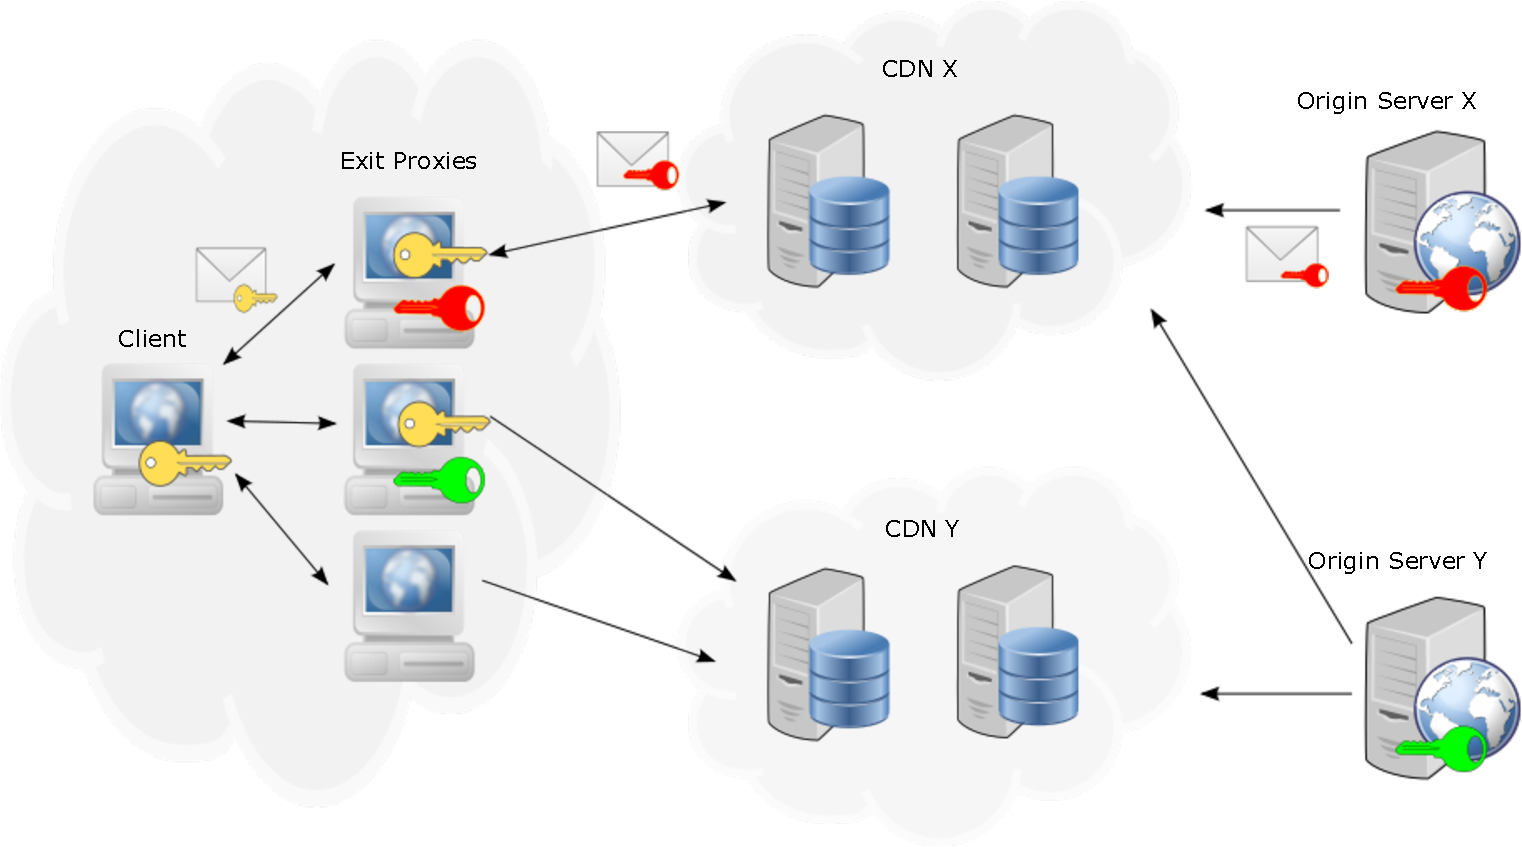
\includegraphics[width=.6\textwidth]{ocdn_overview_updated}
\caption{The relationships between clients, exit proxies, CDNs, and origin servers in 
\system{}.}
\label{fig:ocd_overview}
\end{figure}

\system{} introduces a closed set of proxies (a set of exit proxies).  Using this set of proxies separates the issues of trust and content distribution.  A client no longer needs to trust the CDN, which all other clients would need to trust as well.  Now the client can simply rely on the exit proxies to decouple content distribution from the decision of trust.  

\subsection{Hiding Content}
\label{sec:hiding_content}

We start by discussing how the system components communicate and authenticate one another. 
We introduce shared keys between origin servers and exit proxies, how these keys
are stored, how the exit proxies authenticate themselves to origin servers, and how these 
keys are distributed.

%\begin{table}[t!]
%\footnotesize
%\centering
%\begin{tabular}{ l  p{1.9in} } 
% \multicolumn{1}{c}{\bf Design Decision} & \multicolumn{1}{c}{\bf Function} \\
%\hline \hline
% Shared Keys & {Hides content on cache nodes from CDN.} \\
% Consistent Hashing & {Load balance requests across proxies; ensure no proxy can
% control a given URL.} \\
% Self-Certifying Identifiers & {Authenticates exit proxies to origin servers.} \\
% DNS for Key Sharing & {Allows origin server to share shared keys with exit
% proxies.} \\ \hline
%\end{tabular}
%\caption{Design decisions associated with hiding content from a CDN.}
%\label{tab:setup}
%\end{table}

\textbf{Shared Keys.} 
To prevent an adversary from learning information about content and clients, the CDN must not know anything
about the
content that it is caching.  Therefore, the content {\it and} the associated URL
must be obfuscated
before the CDN sees them.  The content can be obfuscated by encrypting it with a
key that is not
known to the CDN.  Because this must be done prior to caching, the content publisher must 
generate a shared key $k$ to encrypt the content with. Encrypting the content alone does not 
hide all information about content from the CDN; the content identifier, or URL, must also be obfuscated, otherwise the 
CDN can reveal information about which clients accessed which URLs (which is indicative 
of the content).  The obfuscated URL should be fixed and relatively
small; 
these requirements reduce storage requirements and prevent the adversary from guessing
the
URL based on the length of the obfuscated URL.  Unfortunately, using a simple hash allows an 
attacker to guess the content identifier by hashing guesses and comparing with 
the hashes stored in the CDNs caches.  To prevent this attack, the content publisher incorporates the use 
of the shared key $k$ into the hash of the URL by using a hash-based message authentication code 
(HMAC).  Additionally, if the domain supports HTTPS requests, then the content publisher must 
also encrypt the associated certificate with the same key $k$.

The encrypted content and corresponding HMAC are sent to the CDN\footnote{Most CDNs
allow the publisher to
decide on a push or pull model, but \system{} is compatible with either approach.}
and stored in
its caches.  The content publisher then shares the key $k$ with an exit proxy. 
This key allows the 
exit proxy to request encrypted content on behalf of clients by computing the HMAC on the URL.  

\textbf{Consistent Hashing.}
Each exit proxy stores a mapping of URLs to their associated shared key $k$; for example, if 
an origin server has shared key $k$ and publishes a web page {\tt www.foo.com}, then an exit 
proxy will store the mapping of {\tt www.foo.com} to $k$.  The set of exit proxies jointly compute a distributed hash table where the key is the URL ({\tt www.foo.com}) and the value is the 
shared key ($k$).  To assign (key,value) pairs to exit proxies, \system{} uses consistent 
hashing~\cite{karger1997consistent,lewin1998consistent}.  Consistent hashing uses a hash function $H(.)$
to generate identifiers for both exit proxies and for URLs; the identifiers are $H(exit\_ID)$ and $H(URL)$. 
We discuss what $exit\_ID$ is in the next section on Self-Certifying Identifiers.  After the hashes are 
computed, they are mapped to a point on an identifier circle (modulo 2$^{m}$, where $m$ is the length of 
identifier in bits); each URL ($H(URL)$) on the circle is assigned to the first exit proxy ($H(exit\_ID)$) that 
is equal to or follows $H(URL)$ on the circle.  This hashing method is used in \system{} because it provides: 
1)~an evenly distributed mapping of URLs to shared keys among the exit proxies,
2)~a way to prevent an exit 
proxy from choosing which URL it wishes to be responsible for, and 3) a relatively small amount 
of (key,values) to be moved when a new exit proxy is established (or removed).  

\textbf{Self-Certifying Identifiers.} Consistent hashing uses identifiers for both the URLs and 
the exit proxies.  While the identifiers for URLs are straightforward ($H(URL)$), the identifiers for exit 
proxies must provide more information; an exit proxy identifier must be able to prove to an origin server that 
it is the exit proxy that is responsible for the associated URL.  If this validation was not part of \system{}, 
then any (potentially malicious) exit proxy could request the shared key $k$ from any or all origin servers.  To 
prevent a malicious exit proxy from learning any shared key $k$, the proxy must be identified by a self-certifying 
identifer.  This technique was first introduced in a self-certifying file system~\cite{mazieres2000self}; it allows
for other entities (such as origin servers) to certify the exit proxy solely based on its identifier.  The format 
of this identifier ($exit\_ID$) is {\tt IP:hostID}, where {\tt IP} is the exit proxy's IP address and {\tt hostID} 
is a hash of the exit proxy's public key.  A malicious exit proxy cannot \textit{choose} where on the consistent 
hashing ring it sits because it cannot frequently change and re-hash its own IP address (whereas it could re-generate 
a new public key).\footnote{While a malicious exit proxy cannot specifically choose its location on the hashing ring, it 
could recompute a public key until it finds a certain location on the hashing ring.  This is limited by the fact that 
the exit proxy's IP address is part of its identifier, and we assume that the adversary running the exit proxy cannot 
change IP addresses to a value of his choice or in a frequent manner.  A potential attack that an adversary can execute 
on a DHT using a consistent hashing scheme is a Sybil attack, where the adversary runs {\it many} exit proxies to hopefully 
place himself in his desired location on the hashing ring.  We describe countermeasures to a Sybil attack in Section 
\ref{sec:sec}.} When an exit proxy is requesting the shared key $k$ from an origin server, 
it sends its identifier and its public key to the origin server.  The origin server
can then hash the exit proxy's 
public key and verify it against the {\tt hostID}; this action serves as a proof
of the exit proxy's position in the consistent hashing
circle, and thus prevents a proxy from lying about where it lies on the ring (and subsequently lying about which 
URL's shared key it is responsible for).  Note that this $exit\_ID$ is used on the consistent hashing circle as $H(IP):H(hostID)$; the 
$exit\_ID$ must be the same length as $H(URL)$, so the $exit\_ID$ consists of the first half of the bits of $H(IP)$ concatenated 
with the first half of the bits of $H(hostID)$.

\textbf{DNS for Key Distribution.}
We have discussed how shared keys are generated, used, and stored, and here we describe how they are shared.  As previously 
stated, the origin servers generate shared keys and must share them with the (correct) exit proxies.  \system{} uses DNS
to do so.  To retrieve a shared key $k$, an exit proxy sends a DNS query to the origin server's authoritative DNS, and 
it includes its identifier, $exit\_ID$, and its public key in the {\tt Additional Info} section of the query.  The 
authoritative DNS for the origin server validates the exit proxy by hashing the public key and comparing it to the 
second part of $exit\_ID$, and verifying that the exit proxy is responsible for its URL based on the consistent 
hashing circle.  If the verification is successful, then the authoritative DNS sends the shared key $k$ encrypted 
under the exit proxy's public key, \{$k$\}$_{PK_{exit}}$ in the SRV record of the DNS response.  The exit proxy 
extracts $k$ by decrypting with its private key, and stores it in its hash table.

%\begin{table}[t!]
%\footnotesize
%\centering
%\begin{tabular}{ l  p{1.9in} } 
% \multicolumn{1}{c}{\bf Design Decision} & \multicolumn{1}{c}{\bf Function} \\
%\hline \hline
%Spoofed Source Routes & {Hides origin of client request from other
% clients, exit proxies, and CDN.} \\
% Session Keys & {Hides URL and response from other clients.} \\
% Multicast Response & {Allows CDN to return content directly to client without knowing
% the client that requested the content.} \\
% \hline
%\end{tabular}
%\caption{The design decisions associated with content requests and responses, and what these 
%decisions provide.}
%\label{tab:request_response}
%\end{table}

\subsection{Hiding Clients}
\label{sec:hiding_clients}
We make additional design choices that concern the requests that clients initiate
and the responses they receive. We 
introduce session keys for this purpose.

\textbf{Source Routing through Multiple Exit Proxies.}
As previously described, exit proxies query the CDN on behalf of clients, but the
exit proxy
should not be able to learn which client sent which request.  This obfuscation is
accomplished by routing requests through
a series of other exit proxies.  %Each client runs a proxy and is
%also a peer in this system; this 
%peer-to-peer system of clients borrows the 
%protocols used for clients joining, leaving, and learning about other clients from
%the vast literature on peer-to-peer %systems~\cite{monnerat2006d1ht,risson2006stable,zhu2005efficient,gupta2003kelips,lesniewski2008sybil,leong2004achieving}. 
A client routes a request through
intermediate exit proxies by using source routing; when the client generates a request, it also
generates a source route, which includes
the addresses of a set of exit proxies.  The last hop in the source route is the exit proxy that is responsible for the 
shared key $k$ associated with the URL in her request.  The client determines the correct exit proxy by looking up a locally-held URL-proxy map (which is retrieved from a central system that keeps the mapping of URLs to exit proxies).  
It appends this source route to its request and forwards it to the first exit proxy
in the route.  When an intermediate exit proxy receives
a request, she simply forwards it on to the next exit proxy; this continues until the last hop in the source route, which 
is the final exit proxy. 

%To obscure the client that initiated the request, \system{}
%allows each client to spoof source routes; specifically, a client can prepend
%other peers in the route before it initiates a request.  For example, a client
%with identity {\it C} could generate a route to exit proxy {\it E} that looks
%like $C \rightarrow G \rightarrow F \rightarrow E$ and can further obfuscate
%the source of the route by prepending additional clients to the beginning of
%the route as follows: $D \rightarrow A \rightarrow C \rightarrow G \rightarrow
%F \rightarrow E$. Neither {\it G}, {\it F}, nor {\it E} know who the original requestor was; from {\it E}'s point of 
%view, the original requestor could have been {\it D}, {\it A}, {\it C}, {\it G},
%or {\it F}.  Recall from Section \ref{sec:attacker} that our threat model does not 
%include a global passive adversary, and therefore do not prevent an adversary with those capabilities 
%from learning which client issued the request; \system{} does prevent an adversary that is running a 
%client and/or exit proxy from identifying which client issued the request. Using a sequence of 
%peers, or even just knowing that a client {\it can} use a series of peers, hides
%the identity of the client 
%from other clients, exit proxies, and the CDN. 

The option for source routing offers a tradeoff between privacy and performance. Clients interested in prioritizing performance can choose to send requests directly to the correct exit proxy. In such a case, the exit proxy will know the client's identity, but the CDN will not. For more privacy, the client can forward a request through a set of additional exit proxies between it and the final exit proxy. %Lastly, the client could {\it only} prepend other clients' %identifiers but simply %forward the request {\em directly} to the exit proxy; this action provides the same performance benefit as the first mode, but %still offers some %additional privacy benefits. Although the last option would appear to strike the optimal balance between privacy and performance, it %cannot be the only %option because the exit proxy would always know that the true client is the previous hop in the source route. % 
These modes of operation provide clients with different ways to use the system both based on their privacy preferences and the type of content they are requesting.


\textbf{Session Keys for Request and Response Confidentiality.}
In addition to shared keys between origin servers and exit proxies, \system{} uses session keys shared 
between clients and exit proxies.  Session keys provide confidentiality of the requested URL and the 
response.  When the client generates a request, it generates a session key $skey$.
and encrypts 
the URL in her request with this key, which provides \{URL\}$_{skey}$.  The client
must also share this session key
with the exit proxy, so that the exit proxy can learn the plaintext URL and subsequently compute the HMAC to 
query the CDN.  The client encrypts the session key with the exit proxy's public key, resulting in \{skey\}$_{PK_{exit}}$, 
and appends this value as an additional header on the request.  Because her request may be forwarded through a different exit proxy first, this hides the URL of the request from any intermediate exit proxy.

When the last exit proxy receives a request, it first extracts the session
key $skey$ by decrypting it with 
his private key, and then he decrypts the URL with the session key.  This operation
yields the original plaintext
URL. Using the shared key $k$ from the origin server, it can then compute
HMAC$_k$(URL) and forward the request 
to the CDN.  Upon receiving a response from the CDN, the exit proxy then decrypts
the content with the shared key $k$, and
encrypts the content with the session key $skey$ before sending it to the client via the exit proxy that originally forwarded the initial request.
When the client receives the encrypted response, 
she can then decrypt it using $skey$.

%\textbf{Multicast Responses.}
%Using session keys allows for a performance optimization in sending responses back to clients.  Instead of sending 
%the encrypted response from the exit proxy back to the client via the set of peers used in the source route, the exit 
%proxy can send it in a multicast manner to all clients that were on the source route.  The only client that knows $skey$ 
%is the true client that originated the request, therefore none of the other clients can interpret the response, and it reduces the 
%latency for sending the response to the client.  

%\subsection{Incentives for Running \system{}}
%As described in Sections \ref{sec:hiding_content} and \ref{sec:hiding_clients}, \system{} relies 
%on the use of a system of proxies.  These include: 1) client proxies, and 2) exit proxies.  For a client 
%to join the system, they must also run client proxy on his/her machine.  On the other hand, there is no 
%requirement for a client, organization, or company to run an exit proxy; despite this lack of requirement, we 
%believe that both clients and companies have enough incentives to run an exit proxy (or multiple exit proxies).  
%Clients benefit from running an exit proxy because it allows \system{} to perform better in terms of both 
%performance and privacy; when there are more exit proxies, then there is less load put on each exit proxy, and there is a smaller
%chance that an attacker has access to most exit proxies.  Companies benefit from running an exit proxy for similar 
%reasons --- performance and privacy ---, but it could help Internet users access their content quicker (assuming they have 
%content cached by the CDN).    

%\subsection{Incentives}
%While our explanation of the design of \system{} describes a set of proxies that are run by us, but are not 
%trusted; here we describe alternative designs regarding the system of proxies.  The system will work with both a closed, 
%trusted system of proxies, as well as with an open (untrusted) system of proxies.

%{\bf Closed System of Proxies.} While the proxies in \system{} are not trusted, \system{} could 
%use a system of closed and trusted proxies.  There are potential groups or organizations that would 
%support this trusted set of exit proxies, and would be willing (and trusted) to run the exit proxies.  If the exit
%proxies were trusted, then parts of the design of \system{} could be simplified; for example, if proxies 
%were trusted, then \system{} would not need to hide the identity of clients from the exit proxies, and could 
%remove spoofed source routes from the design.  The primary drawback of this approach is finding an organization 
%that everyone could trust to run the exit proxies.  

%{\bf Open System of Proxies.} In \system{}, exit proxies are not 
%trusted with client identities and information, which removes the need to find a universally trustworthy 
%organization.  In an alternative approach, \system{} could use a completely open system of proxies that are 
%untrusted, which would allow anyone (clients, companies, etc.) to run an exit proxy.  
%The addition of an exit proxy follows the protocol in consistent hashing for when a new node 
%joins; some keys would be transferred to the new exit proxy, and clients' mapping of 
%exit proxies will be updated.  This allows for the load to be split among more proxies and 
%increases the geographic diversity of the exit proxies.  

%\subsection{Design Enhancements}

%We discuss possible enhancements to \system{}'s basic design.

%\textbf{Multiple CDNs.}
%While describing the design decisions that went into \system{}, we referred to a single CDN for 
%simplicity.  In reality, \system{} allows for many CDNs to participate;
%distributing content across
%multiple CDNs could provide additional privacy. Origin servers can also take advantage
%of multiple CDNs.

%\textbf{Encoding URLs.}
%As described earlier, each URL is obfuscated by using a HMAC and then stored on the CDN.  An adversary 
%could potentially correlate a URL's popularity with its access patterns.  To prevent this, \system{} allows 
%origin servers to generate multiple different encodings of its URLs, such that HMAC$_k$(enc$_1$(URL)) $\neq$ 
%HMAC$_k$(enc$_2$(URL)).  Each origin server could produce $n$ different encodings of popular URLs, such that 
%the popularity distribution seen by an adversary is a uniform distribution of URL requests across all URLs.  

%\textbf{DHT Replicas.}
%Each exit proxy's hash table can be replicated by another (or many other) exit proxies, spreading the burden across multiple proxies. This behavior would %provide less load per exit proxy, as well as redundancy in case of failures.  Additionally, 
%the CDN can cache the content associated with a given URL at more than one cache
%node;
%if only one exit proxy is responsible for a given URL's content, then it would likely only be cached at 
%cache node closest to the exit proxy.  Having multiple exit proxies responsible for a URL's content 
%helps decrease the load on the proxies while maintaining some of the performance benefits of a CDN.

%\textbf{Hybrid OCDN/CDN Designs.}
%Different origin servers have different needs, and each origin server might 
%have different needs for different content.  The design of \system{} allows origin servers
% to publish some of their content on \system{} and some on other CDNs.  
%This is useful in a case where some content is more sensitive, while other content needs 
%better performance.

%\textbf{Pre-Fetch DNS Responses.} 
%One way to increase the performance of \system{} is to pre-fetch DNS responses at 
%the exit proxies.  This would allow the exit proxy to serve each client request faster 
%because it would not have to send as many DNS requests.  Pre-fetching DNS responses would 
%not take up a large amount of space, but it also would not be a complete set of all DNS 
%responses.  Additionally, if the CDN moves content between cache nodes, then DNS 
%response must also change; therefore, the pre-fetched DNS responses should have a lifetime 
%that is shorter than the lifetime of the content on a cache node.

%\textbf{Privacy vs. Performance Tradeoffs.}
%There are two different modes that \system{} can operate in, where one provides better 
%performance, and the other provides better privacy.  In the first mode, the client can 
%choose to send a request directly to the exit proxy.  
%
%In this case, the exit proxy might be able to discover the identity of the client,
%but the CDN would still not be able to map a request to the client that made the
%request.
%Alternatively, the client can forward a request
%through a set of peers before it reaches the exit proxy.  In this case, the client
%can 
%prepend other clients' identifiers (as previously described) to make it appear as
%though the request came from
%a different client.  This action further obscures the relationship between the client
%and the request.  As another option, the client could {\it only} prepend
%other clients'identifiers but simply forward
%the request {\em directly} to the exit proxy; this action provides the same performance
%benefit as the first
%mode, but still offers some additional privacy benefits.  Although the last option
%would appear to strike the optimal balance between privacy and performance, it cannot
%be
%the only option because the exit proxy would always know that the true client is the previous hop 
%in the source route.  These modes of operation provide clients with different ways to use 
%the system both based on their privacy preferences and the type of content they are requesting.


\section{\system{} Protocol}
\label{sec:protocol}
Based on the design decisions discussed in the previous section, we specify the 
steps taken to publish and retrieve content in \system{}.

\subsection{Publishing Content}
In order to publish content such that the CDN never sees the content, the publisher 
must first obfuscate her content, as described in Section \ref{sec:obfuscate_content}. 
Figure \ref{fig:publishing} shows the steps taken when publishing content.

\begin{figure*}[t]
    \centering
    \begin{subfigure}[h]{0.5\textwidth}
        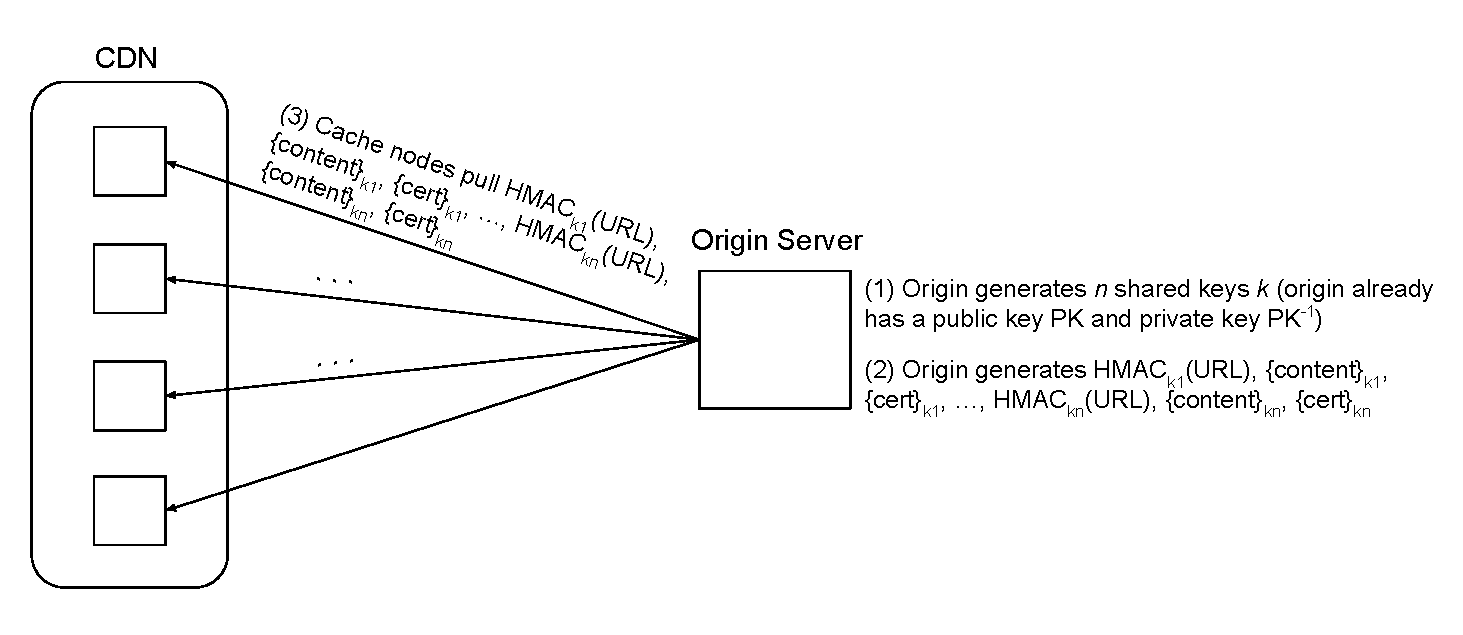
\includegraphics[width=\textwidth]{publishing_content}
    \end{subfigure}%
    \begin{subfigure}[h]{0.5\textwidth}
        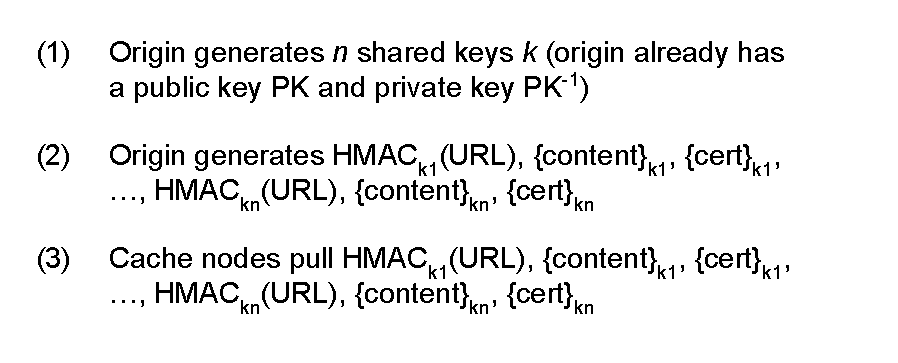
\includegraphics[width=\textwidth]{Publishing_steps}
    \end{subfigure}
    \caption{Step-by-step instructions on how content is published in \system{}.}
    \label{fig:publishing}
\end{figure*}

The most important step in content publishing is obfuscating the data.  We assume that the origin 
server already has a public and private key pair, as well as a certificate.  To obfuscate the data 
the origin server will need to generate $n$ shared keys, where $n$ should be between 1 and the number of 
proxies.  We reason about the security of different values of $n$ in Section \ref{sec:analysis}.  

Once all keys are established, the publisher must first pad the content to the same size for some 
range of original content sizes (i.e., if content is between length x and y, then pad it to length 
z).  This content padding is done to hide the original content's length, as it may be identifiable 
simply by its length.  After content is padded, then the content is divided into fixed size blocks and padded to 
some standard length.  Then for each shared key $k$, each block is encrypted using the shared key, 
such that there are $n$ sets of encrypted blocks. As long as the CDN does not have access to any 
of the $n$ shared keys, then the CDN cannot see what content it is caching.  

Now that the content is obfuscated, the publisher must also obfuscate the content's identifier.  To do so, 
she computes the HMAC of the URL using the shared key $k$, for each shared key.

Once the identifier and the content replicas are obfuscated $n$ times (with $n$ keys), they can be pushed to the 
CDN.  To increase reliability, performance, and availability, the publisher can push the content to 
multiple CDNs; a publisher can use a service, such as Cedexis~\cite{cedexis}, to load balance between 
CDNs.  We discuss the use of multiple CDNs more in Section \ref{sec:partial} on \system{} in 
partial deployment.  Note that each proxy will only be able to fetch a specific replica of the content, that is a 
specific \{content\}$_{kn}$ for the $n^{th}$ shared key that it holds.  We discuss the security and performance trade offs 
associated with differing numbers of shared keys and proxies in Sections \ref{sec:analysis} and \ref{sec:performance}.

%\begin{enumerate}
%\item Origin generates n shared keys k (origin already has a public key PK and private key PK$^{-1}$)\footnote{$n$ such that $1 < n < |proxies|$} 
%\item Origin generates HMAC$_{k1}$(URL), \{content\}$_{k1}$, , \{cert\}$_{k1}$, ..., HMAC$_{kn}$(URL), \{content\}$_{kn}$, \{cert\}$_{kn}$
%\item Cache node pulls HMAC$_{k1}$(URL), \{content\}$_{k1}$, , \{cert\}$_{k1}$, ..., HMAC$_{kn}$(URL), \{content\}$_{kn}$, \{cert\}$_{kn}$\footnote{For more security and reliability, cache nodes from different CDNs can pull this data.  Additionally, an origin server can use something like Cedexis to load balance between CDNs.}
%\end{enumerate}

\subsubsection{Updating Content}
For a content publisher to update content, she must follow similar steps as described in publishing content.  
Once she has updated the content on her origin server, she must obfuscate it using the same steps: 1) padding the 
original content length, 2) divide the content into fixed size blocks, and 3) encrypt $n$ copies of the content blocks 
with each of the shared keys.  Because she is updating the content (as opposed to creating new content), the 
obfuscated identifier will remain the same.  She must 
retain a copy of the obfuscated old content until after the new content has been updated on the CDN; this is to prove 
that the old content owner is the same as the new content owner.  Only the origin and the proxy, both of which are 
outside the CDN, know the old obfuscated content, so an attacker cannot update the content that belongs to 
a legitimate publisher.  The publisher must present the old obfuscated content to the CDN in order to also push 
her new obfuscated content to the CDN. 

\subsection{Retrieving Content}
The steps taken for an end-user to retrieve a web page that has been cached by \system{} are shown in Figure \ref{fig:retrieving}.  
The end-user must first configure her browser to use an \system{}-designated proxy.  A client is assigned to a 
specific proxy, and she configures her browser to use the assigned proxy.    Then, once she sends a request for a 
web page, it goes to the proxy via a TLS connection.\footnote{Comment: Add blinding here such that client1's request for foo.com and 
client2's request for foo.com looks different as it goes from the client to the proxy.  So the proxy must be able to un-blind 
the request.}  The proxy then resolves the domain using it's local resolver, which will 
redirect it to the CDN's DNS resolver. 

In order for the proxy to generate the obfuscated identifier to query the edge server for the correct content, 
it must have one of the $n$ shared keys that the origin server generated and obfuscated the content and identifier 
with.  The origin server publishes the shared key encrypted with the proxy's public key\footnote{Additionally, the origin server 
can learn the proxy's public key via DNS as well; for example, the proxy can publish it's public key in the DNS SRV record.} in the DNS SRV record; therefore, 
when the proxy sends a DNS request to the origin server's authoritative DNS server, it will receive the encrypted shared 
key, which it can decrypt with it's private key.  

Now that the proxy has obtained a shared key from the origin server, it can generate the obfuscated content identifier based 
on the request the client sent.  It computes the HMAC of the URL with the shared key.  The proxy then 
sends the (obfuscated) request to the edge server, where the CDN locates the content associated with the identifier.  The CDN returns 
the associated obfuscated content, which we recall is the fixed size blocks encrypted with the same shared key that the identifier was 
obfuscated with.  The proxy can decrypt the content blocks with the shared key from the origin server, assemble the blocks, and strip any 
added padding, to reconstruct the original content.\footnote{Comment: Proxy can cache content in times of flash crowd to minimize correlation attacks if a provider has encrypted and unencrypted content on the same CDN.  This raises the issue of charges for the origin (the CDN can’t charge as much if edge servers don’t see as many requests for the origin) --- RFC 2227 describes a solution for this~\cite{rfc2227}.}  Finally, the proxy returns the content to the client over TLS.  

%\begin{enumerate}
%\item Send GET foo.com request to proxy using TLS connection\footnote{Include some form of blinding here such that client1 and client2 request the same URL, but the contents of step 1 look different by adding some randomness at the client, and that the proxy can remove \url{https://en.wikipedia.org/wiki/Blinding_(cryptography)} --- this prevents a malicious CDN from running a client and sending requests to learn things about other clients.}
%\item DNS lookup from proxy for foo.com\footnote{This DNS info could be prefetched on the proxy, which would provide some optimization.}
%\item CDN DNS lookup for a19.akamai.net (some Akamai ID that represents foo.com)
%\item Proxy sends DNS request to origin’s authoritative server, and the origin publishes \{k\}$_{PK_{proxy}}$ in the SRV record.  Then the proxy decrypts the shared key with his own private key.\footnote{The origin can learn the proxy’s public key via DNS.}, \footnote{The shared keys are updated every X amount of time, so this fetching of the shared key needs to happen regularly.}
%\item Proxy generates GET HMAC$_k$(URL) request
%\item Proxy sends request to cache node
%\item Cache node returns \{content\}$_k$, \{cert\}$_k$ to proxy.  Proxy decrypts and validates the cert.  Once the cert is validated, proxy decrypts the content with origin server’s shared key.\footnote{Proxy can cache content in times of flash crowd to minimize correlation attacks if a provider has encrypted and unencrypted content on the same CDN. This raises the issue of charges for the origin (the CDN can’t charge as much if edge servers don’t see as many requests for the origin) --- RFC 2227 describes a solution for this: Simple Hit-Metering and Usage-Limiting for HTTP.}
%\item Proxy returns decrypted content to client (using TLS)
%\end{enumerate}

\begin{figure*}[t]
    \centering
    \begin{subfigure}[h]{0.5\textwidth}
        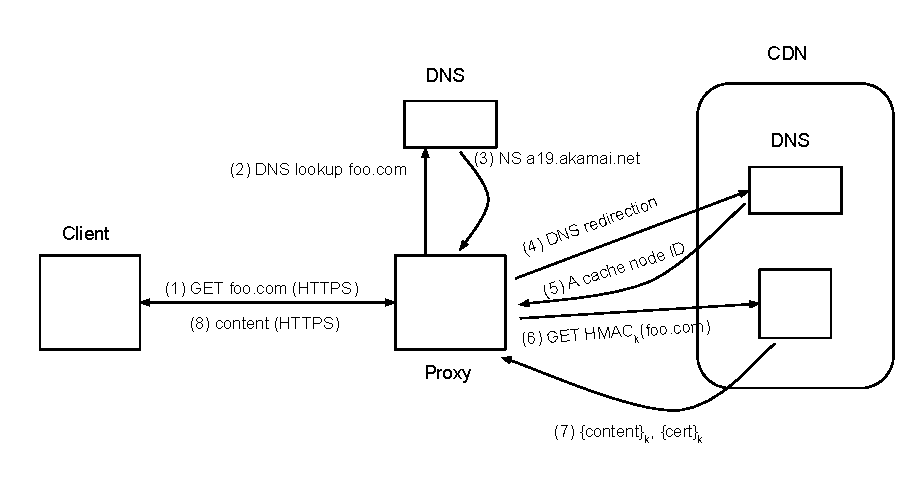
\includegraphics[width=\textwidth]{retrieving_content}
    \end{subfigure}%
    \begin{subfigure}[h]{0.5\textwidth}
        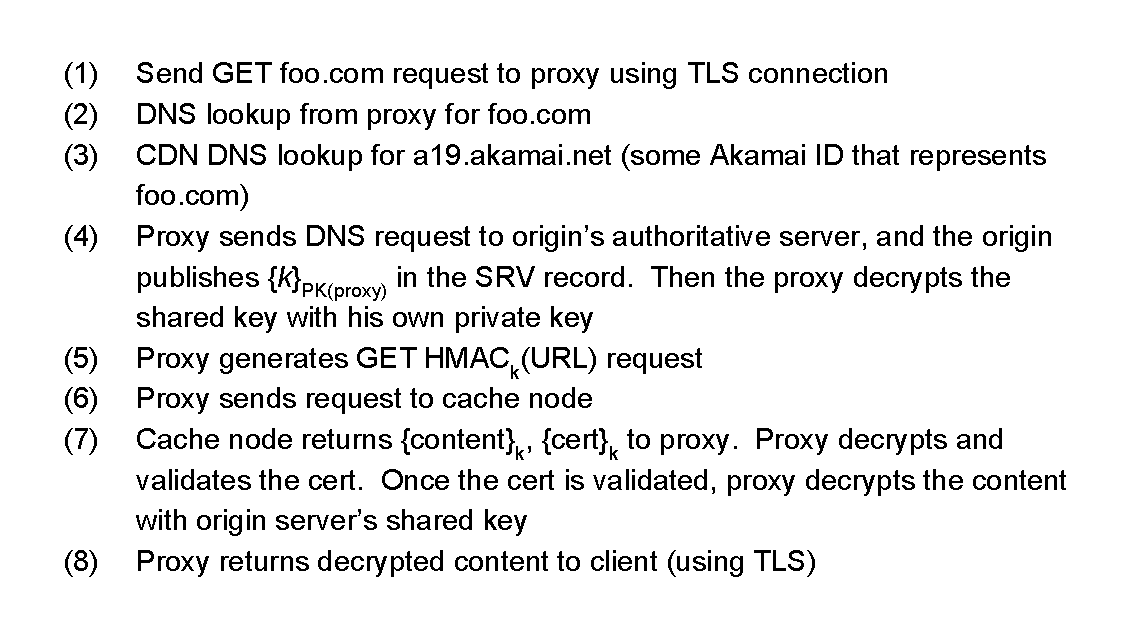
\includegraphics[width=\textwidth]{Retrieving_steps}
    \end{subfigure}
    \caption{Step-by-step instructions on how content is retrieved in \system{}.}
    \label{fig:retrieving}
\end{figure*}

\subsection{Partial Deployment}
\label{sec:partial}
\system{} should be partially deployable in the sense that if only some of the content publishers participate or only some of the CDNs participate, then 
the system should still provide protections.  We have two different partial deployment plans, and both provide protections for those 
publishers, CDNs, and clients that use \system{}. 

{\bf Plan 1.}
One option for deploying \system{} is to ensure there is some set S of content publishers the participate fully in the 
system.  These publishers obfuscate their content, identifiers, and certificates, and most importantly, only have 
obfuscated data stored on the CDNs cache nodes.  Recall that there are n shared keys, resulting in n replicas of the 
content that {\it appear} to the CDN as different content (because each replica is encrypted with a different key).  This 
allows the minimum set of publishers S to be relatively small.  We discuss the security tradeoffs with different 
values of S in Section \ref{sec:analysis}.  This partial deployment plan protects the set of content publishers S and it 
partially protects the privacy of the clients accessing the content created by the set of publishers S.  It does not 
protect the clients' privacy as completely as full participation of all publishers in \system{} because the CDN can 
still view cross site browsing patterns among the publishers that are not participating. It is important to note though, that 
because the clients are behind proxies, the CDN cannot individually identify users.  The CDN can attribute requests to proxies, but 
not to clients.  

{\bf Plan 2.} 
It is reasonable to believe that some content publishers are skeptical of \system{} and prioritize performance 
and availability.  Therefore, they should have the option to gradually move towards full participation by pushing 
both encrypted and plaintext content to the CDN.  In this partial deployment plan, we see some set of publishers 
fully participating with only encrypted content, some other set of publishers partially participating with both 
encrypted and plaintext content, and some last set of publishers that are not participating.  Unfortunately, if 
a publisher has both encrypted and plaintext content at a cache node, and some event causes a flashcrowd --- 
the CDN sees a significantly larger spike in accesses to certain content --- then the CDN can correlate the access 
spike on encrypted and plaintext content for the same publisher.  In order to prevent this deanonymization of the 
content publisher, we can utilize multiple CDNs.  The publisher can spread replicas over different CDNs such that 
the encrypted replicas are on one CDN and the plaintext replicas are on a different CDN.  In this case the publisher 
is not susceptible to flashcrowds correlations and can still partially join the system.

\subsection{Optimizations}
\label{sec:optimizations}
While there are some optimizations that CDNs typically perform today that would not be possible with \system{}, the architecture 
of \system{} allows for new optimizations that are not possible in existing CDNs.  Here we first outline some ways in which \system{} 
can be optimized in terms of performance, and then we point out what performance enhancements CDNs would not be able to do with 
\system{}.

{\bf Pre-Fetch DNS Responses.} One way to increase the performance of \system{} is to pre-fetch DNS responses at 
the proxies.  This would allow the proxy to serve each client request faster because it would not have to send 
as many DNS requests.  Pre-fetching DNS responses would not take up a large amount of space, but it also 
would not be a complete set of all DNS responses.  Additionally, if the content is moved between cache nodes 
at the CDN, then DNS response must also change; therefore, the pre-fetched DNS responses should have a 
lifetime that is shorter than the lifetime of the content on a cache node.

{\bf Load Balance Proxy Selection.} As the proxy performs a number of operations on the client's behalf, it 
runs into the possibility of being overloaded.  With \system{}, a client can be redirected to different 
proxies based on load; this can be implemented with a PAC file, which allows 
a client to access different proxies for different domains.  In addition to being a performance benefit, 
this could also prevent a country from blocking the set of proxies that all of the country's citizens use; if 
this occurs, then the citizens can be redirected to a different proxy.   

On the other hand, CDNs become more limited in some of their actions when following \system{}'s design.  For example, 
many CDNs perform HTTPS re-writes on content that they cache, but this can only be done if the CDN has access to the 
decrypted content.  Similarly, the CDN needs the decrypted content to perform minimizations on HTML, CSS, and Javascript 
files.  Any algorithms used internally to distribute content to certain caches based on what the content is can no longer 
be used in \system{} because the CDN does not know what the content is. 

\section{Implementation}
\label{sec:implementation}

We have implemented a prototype of \system{} to demonstrate its feasibility and 
evaluate its performance.  Our implementation allows a client to send a request 
for content through an exit proxy, which will fetch the corresponding 
encrypted content.  Figure \ref{fig:impl} shows our prototype; the solid line represents
how \system{} communicates between the components, and the dotted line represents how 
a traditional CDN would communicate in our prototype.  Here we will discuss each component---client, exit proxy, 
and CDN---separately, and how they fit together.

\begin{figure}[t]
\centering
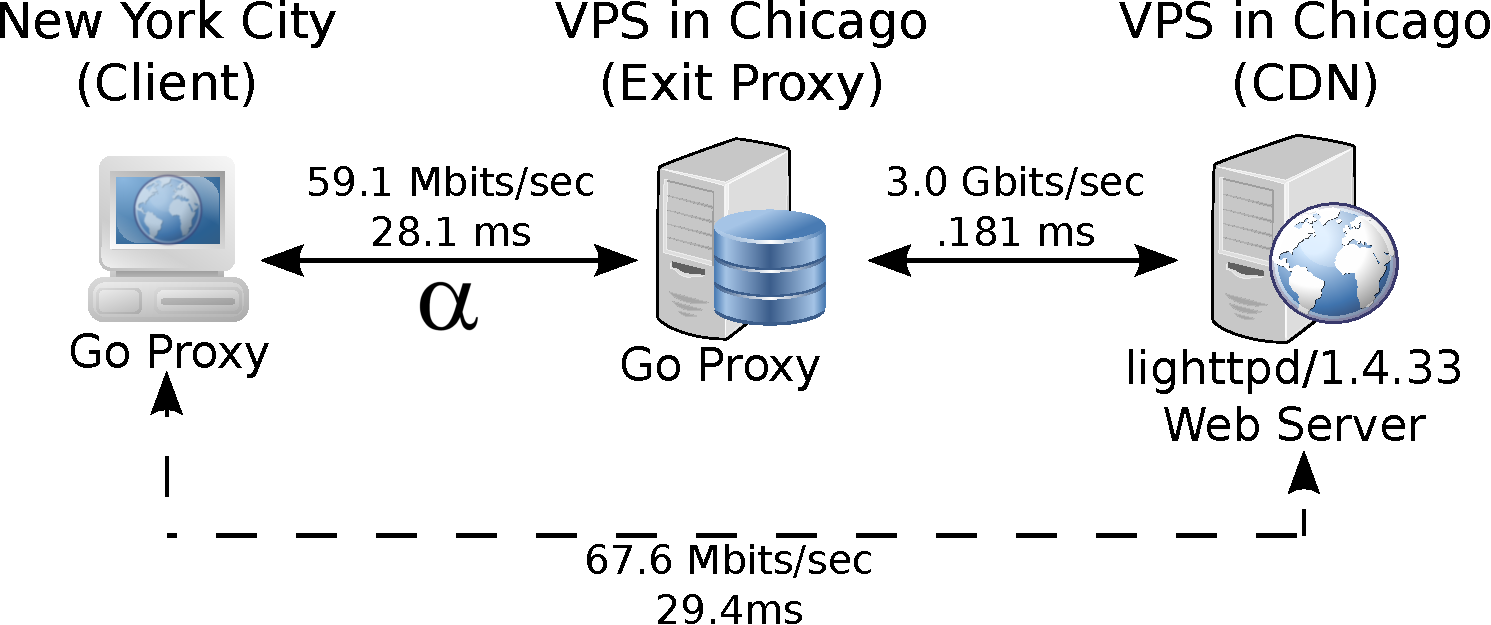
\includegraphics[width=.375\textwidth]{implementation2}
\caption{The implementation of our \system{} prototype.  The solid line represents
how \system{} communicates between the components; the dotted line represents how 
a traditional CDN would communicate. $\alpha$ represents the latency between the client 
and the exit proxy; we simulate additional clients on this path by increasing $\alpha$.}
\label{fig:impl}
\end{figure}
\begin{figure*}[t!]
%\vspace{-2mm}
  \begin{minipage}[t]{.31\linewidth}
    \centering
     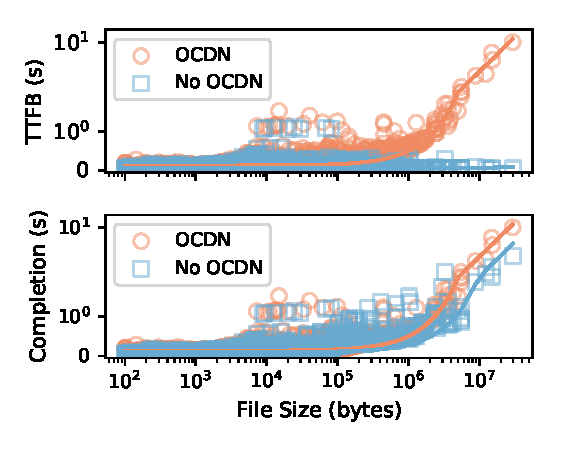
\includegraphics[trim={10 15 10 12},clip,width=\textwidth]{combined}
    \caption{Time to first byte and time to complete a request with and without \system{}.}
    \label{fig:completion}
  \end{minipage}
  \hfill
  \begin{minipage}[t]{.29\linewidth}
    \centering
    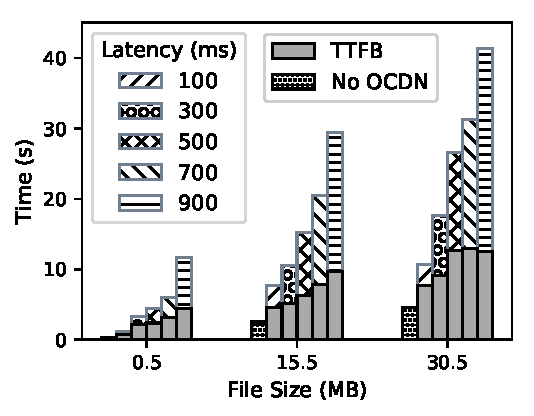
\includegraphics[trim={7 0 10 5},clip,width=\textwidth]{Latency_withoutzero_2}
    %\vspace{-10mm}
    \caption{Time to first byte and time to complete a request with varying the file size and latency.}%; this latency corresponds to $\alpha$ in Figure \ref{fig:impl}.}
    \label{fig:latency}
  \end{minipage}
  \hfill
  \begin{minipage}[t]{.35\linewidth}
    \centering
    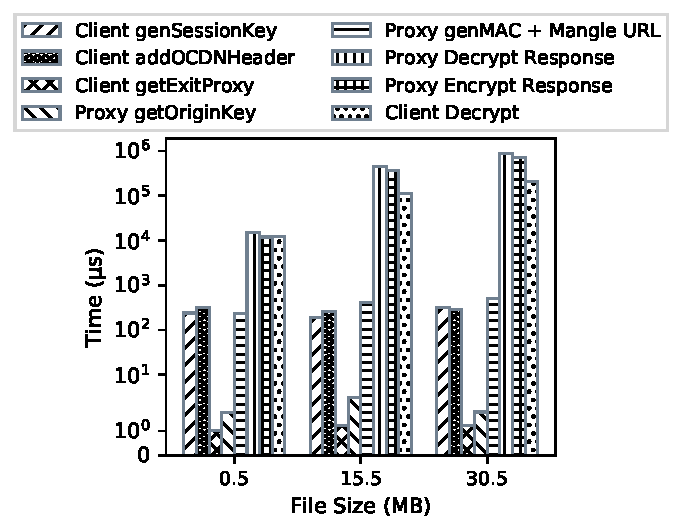
\includegraphics[trim={7 8 7 7},clip,width=\textwidth]{loggrouped_2}
\caption{Overhead of different operations performed by \system{}.}
\label{fig:overhead2}
  \end{minipage}
\end{figure*}


\textbf{CDN.} As the design for \system{} requires encrypted content and identifiers
to be stored in the CDN, we cannot request content from real-world CDNs without
establishing a business relationship with an existing CDN ourselves. Additionally,
we must evaluate the performance of \system{} in comparison to the same content, cache locations, etc., so 
we set up a data storage server.  This server is run on a Virtual Private Server
(VPS) located in
Chicago, USA.  To serve content, we set up a web server on this VPS machine.  To generate 
plaintext web content, we used Surge~\cite{barford1998generating}, which allows us 
to generate a set of files that are representative of real-world web server file distributions.  
In \system{}, the files are encrypted with a shared key $k$ and the obfuscated file name is the 
HMAC$_{k}$(file name).  We use AES with 256-bit keys for the shared key and SHA-256
for the 
hash function.  Both the plaintext files and encrypted files are stored on this web server, and 
for the purposes of evaluating our prototype, act as a CDN in \system{}.

\textbf{Exit Proxy.} The exit proxy is the component that queries the CDN for
encrypted
content on behalf of a client.  We have implemented a web proxy in Go; this proxy
runs on
a different VPS machine in Chicago, USA.  In addition to proxying web requests, the exit 
proxy also provides cryptographic functionality.  When receiving a request, it rewrites
the URL in the request to be the HMAC$_{k}$(URL), and it parses the headers to retrieve a 
specific header, {\tt X-OCDN}, which contains the client's session key encrypted
under the exit
proxy's public key.  Our implementation uses 2048-bit RSA for asymmetric encryption.  After 
decrypting the session key, it stores it in memory for use on the response.  When 
it receives a response from the CDN, it decrypts the content with the shared key $k$, and 
subsequently encrypts it with the session key (both using AES 256-bit encryption).  The 
exit then forwards the response onto the client proxy.

\textbf{Client Proxy.} The client runs a local proxy, which performs cryptographic computations on behalf of the client that is
requesting
content.  This proxy uses the same implementation as the exit proxy, but provides 
different cryptographic functions on the requests and responses.  When a client makes 
a request, the client proxy generates a session key  (AES 256-bit) and looks up the correct exit proxy's 
public key.  The client proxy then adds a header to the request, 
where X-OCDN is the key, the encrypted session key is the value.  The client then forwards this on to the 
exit proxy.  When the client receives a response from the exit proxy, it must decrypt the content 
with the session key it originally generated.   

\section{Security Analysis}
\label{sec:sec}
We analyze and discuss how \system{} addresses different attacks.  Table \ref{tab:sec_table} 
shows what security and privacy features \system{} provides in comparison to other related 
systems.

\begin{table}[t!]
\centering
\begin{tabular}{| l | l | l | l |} 
\hline
 {} & Preserves  & Preserves   & Protects \\ 
 {} & Integrity & Confidentiality & Client\\
 {} & at CDN & at CDN & Identity \\
\hline
 Stickler~\cite{levy2015stickler} & \checkmark & {} & {}\\ 
 Repeat \& Compare~\cite{michalakis2007ensuring} & \checkmark & {} & {}\\
 OCDN & {} & \checkmark & \checkmark\\
 Tor~\cite{dingledine2004tor} & {} & {} & \checkmark \\
\hline
\end{tabular}
\caption{The security and privacy features offered by related systems.  To our knowledge, 
\system{} is the first to address confidentiality at the CDN.}
\label{tab:sec_table}
\end{table}

{\bf Popularity Attacks.}  An attacker that has requested or otherwise 
gained access to CDN cache logs can learn information about how often 
content was requested.  Because not all content is requested uniformly, the 
attacker could potentially correlate the most commonly requested content with 
very popular webpages.  While this does not allow the CDN to learn which 
clients are accessing the content, it can reveal information about what content 
is stored on the CDN cache nodes.  \system{} handles this type of attacker by making 
the distribution of content requests appear uniform.  The content publisher (of popular 
content) generates multiple shared keys 
and encrypts their content under each key, such that they have multiple, different-looking 
copies of their content.  All of the content copies are pushed to the CDN and each key is 
shared with the exit proxies.\footnote{This also provides load balancing for exit proxies 
that hold originally held the sole key for the popular webpage, but this is now distributed 
across multiple exit proxies.}  Now, the popular content does not appear as popular, 
and it makes difficult for an attacker to infer the popularity of the content.

{\bf Chosen Plaintext Attacks.} An attacker could attempt to
determine whether a particular URL was being accessed by sending requests
through specific \system{} proxies and requesting access to the CDN cache logs, 
which contain the corresponding obfuscated
requests and responses. Blinding the clients' requests
with a random nonce that is added by the proxy should prevent against this
attack. We also believe that such an attack reflects a stronger attack: from a
law enforcement perspective, receiving a subpoena for {\em existing} logs and
data may present a lower legal barrier than compelling a CDN to attack a
system.

{\bf Spoofed Content Updates.} Because the CDN cache
nodes do not know either the content that they are hosting or the URLs
corresponding to the content, an attacker could masquerade as an origin server
and could potentially push bogus content for a URL to a cache node. There are
a number of defenses against this possible attack. This simplest solution is
for CDN cache nodes to authenticate origin servers and only accept updates
from trusted origins; this approach is plausible, since many origin servers already
have a corresponding public key certificate through the web PKI hierarchy.  An additional
defense is to make it difficult for to discover which obfuscated URLs correspond
to which content that an attacker wishes to spoof; this is achievable by design.
A third defense would be to only accept updates for content from the same origin
server that populated the cache with the original content.

{\bf Flashcrowds.}  A flashcrowd is large spike in traffic to a specific web page.  An attacker 
could see that some content on the CDN has just seen a surge in traffic and correlate that with 
other information (for example, major world events).  This leaks information about what the content the 
CDN is caching.  Fortunately, the design of \system{} can defend against this type of inference attack.  
The exit proxy can cache content in time of a flashcrowd, such that the CDN (and therefore the attacker) 
does not see the surge in traffic.  

\begin{figure*}[t!]
\vspace{-2mm}
  \begin{minipage}[t]{.31\linewidth}
    \centering
     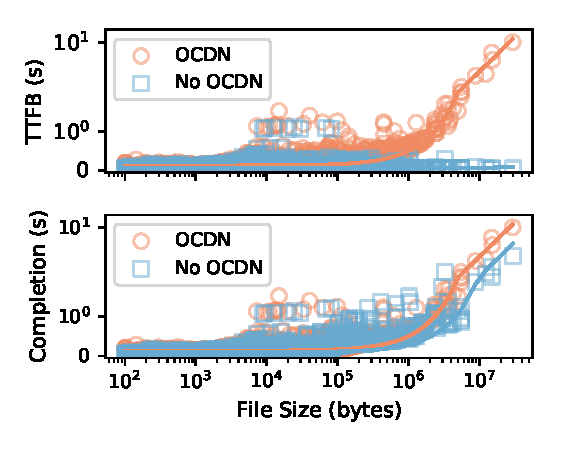
\includegraphics[trim={10 15 10 12},clip,width=\textwidth]{combined}
    \caption{Time to first byte and time to complete a request with and without \system{}.}
    \label{fig:completion}
  \end{minipage}
  \hfill
  \begin{minipage}[t]{.29\linewidth}
    \centering
    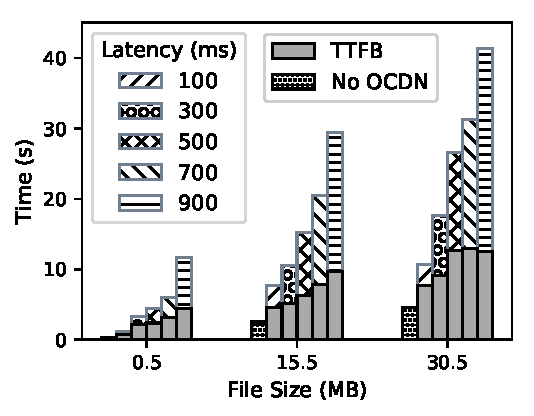
\includegraphics[trim={7 0 10 5},clip,width=\textwidth]{Latency_withoutzero_2}
    %\vspace{-10mm}
    \caption{Time to first byte and time to complete a request with varying the file size and latency.}%; this latency corresponds to $\alpha$ in Figure \ref{fig:impl}.}
    \label{fig:latency}
  \end{minipage}
  \hfill
  \begin{minipage}[t]{.35\linewidth}
    \centering
    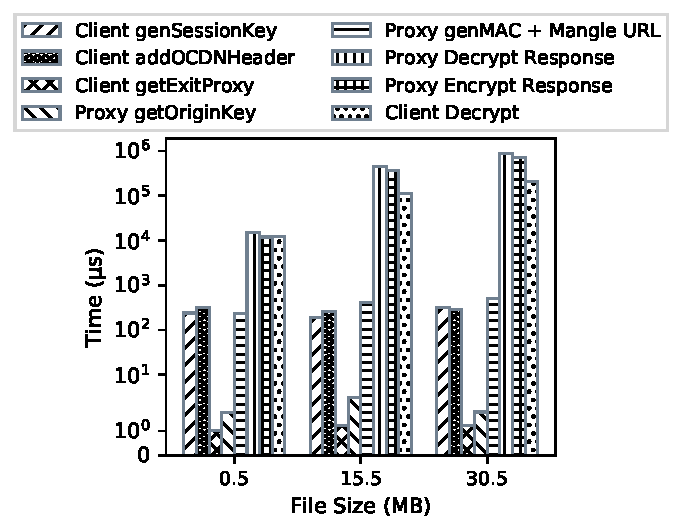
\includegraphics[trim={7 8 7 7},clip,width=\textwidth]{loggrouped_2}
\caption{Overhead of different operations performed by \system{}.}
\label{fig:overhead2}
  \end{minipage}
\end{figure*}


\section{Performance Analysis}
\label{sec:performance}
To evaluate how much overhead is caused by \system{} we measure the performance 
of \system{}.  In addition to understanding the latency and overhead produced by the 
system, we also discuss the scalability of the design and show how \system{} scales 
well with an increasing number of clients.

\subsection{\system{} Overhead}
For measuring performance characteristics of \system{}, we use the implementation 
described in Section \ref{sec:implementation}.  Figure \ref{fig:impl} shows 
how our measurements reflect \system{} (solid line) and a traditional CDN (dotted 
line).  

Figure \ref{fig:completion} shows the time to first byte (TTFB) and the time for both \system{} and 
without \system{}.  We can see the the TTFB using \system{} grows linearly with 
file size, whereas without \system{} TTFB remains fairly constant.  Interestingly, 
we can see that there are some fixed time operations that \system{} performs, which 
is visible by looking at the smaller file sizes. Completion time grows linearly with file size, but for both \system{} and without \system{}; while both follow the 
same pattern, the time to complete requests is, as expected, longer using \system{} as it performs many cryptographic operations and proxies traffic between the client and the CDN.

%\begin{figure}[t!]
%\centering
%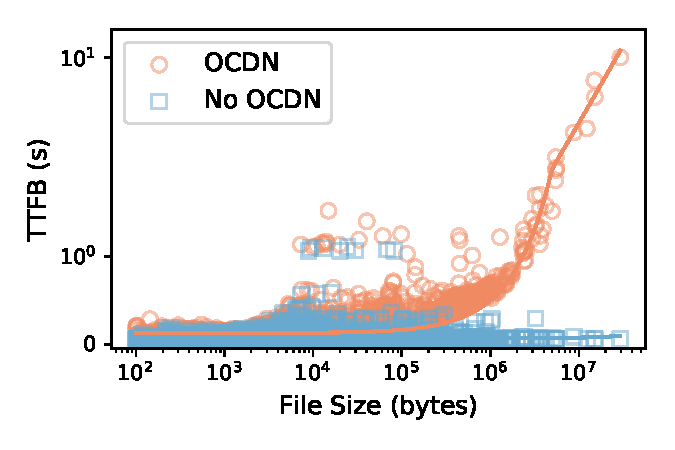
\includegraphics[width=.4\textwidth]{TTFB}
%\caption{Time to first byte measurements with and without \system{}.}
%\label{fig:ttfb}
%\end{figure}  

%\begin{figure}[t!]
%\centering
%\includegraphics[width=.4\textwidth]{completion}
%\caption{Time to complete a request with and without \system{}.}
%\label{fig:completion}
%\end{figure}

As described in Section \ref{sec:implementation}, our prototype included only a single client, but 
our design allows for a client to proxy her request through additional clients.  To simulate this, we 
add latency between the client and the exit proxy, and measure both the TTFB and time to complete a request 
when there are different values of latency, which represent different numbers of clients on the path between the 
original client and the exit proxy.  Figure \ref{fig:latency} shows the results for three different file sizes. The 
bottom portion of each bar in the graph shows the TTFB, and the top portion shows the additional time needed 
to complete the request.  As expected, the TTFB grows much slower as file size and latency increase; completion time 
grows more quickly than TTFB as the file size and latency increase.   

%\begin{figure}[t!]
%\centering
%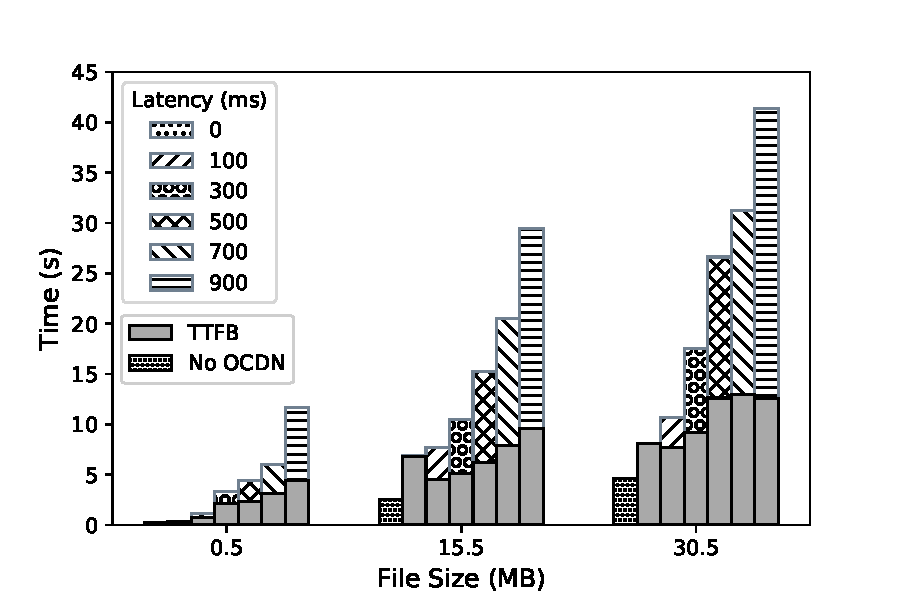
\includegraphics[width=.4\textwidth]{Latency_withzero}
%\caption{Time to first byte and time to complete a request with varying the file size and latency; this latency 
%correspondes to $\alpha$ in Figure \ref{fig:impl}.}
%\label{fig:latency}
%\end{figure}

Finally, we measure the performance overhead of the individual operations used in
\system{}; figure \ref{fig:overhead2} shows
the overhead of different components of the system for three different file sizes.  We can see that some of the fixed cost/time 
operations include the client locally looking up the correct exit proxy to use for a given URL and the exit proxy generating the 
HMAC$_{k}$(URL).  The operations that have the most overhead and continue to grow with the size of the file are the exit proxy decrypting 
the response with the shared key $k$, the exit proxy encrypting the response with the session key $k_{session}$, and the client 
decrypting the response with the session key $k_{session}$.

%\begin{figure}[t!]
%\centering
%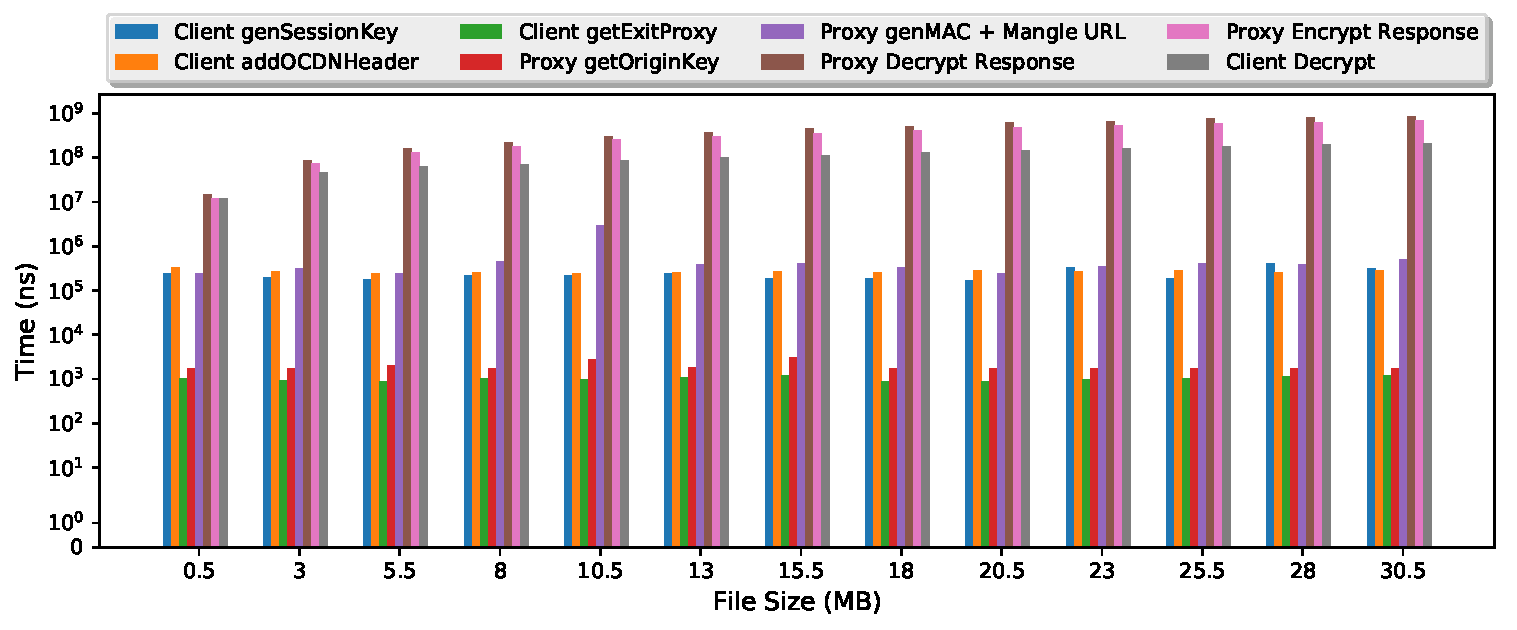
\includegraphics[width=.34\textwidth]{loggrouped}
%\caption{Overhead of different operations performed by \system{}.}
%\label{fig:overhead2}
%\end{figure}

\subsection{Scalability}
\label{sec:scalability}
For evaluating performance, we are also concerned with how well \system{} will scale with more users 
and more URLs.  In particular, we need to reason about how much load is put on the exit proxies as the 
system grows; clients do not bare much load in the system as they simply proxy requests and the CDN is designed 
to handle high numbers of requests, therefore, we limit our scalability analysis to the exit proxies.  

As previously mentioned, we balance load among the proxies by using consistent hashing to assign URLs to 
exit proxies.  \system{} can additionally distribute load by replicating exit proxies, meaning that two exit proxies can 
have the same distributed hash table of shared keys.  This way, both exit proxies can accept requests from clients for 
the URLs they are responsible for.  Also worth noting is that the exit proxy is only recieving requests for the content 
corresponding to the shared keys it contains.  Therefore, as the number of clients grow, the exit proxy is still only responsible 
for its set of shared keys and subsequent URLs.  And as the number of URLs increase, the additional load per proxy is 
still low because of the load balancing properties of consistent hashing.  We also discuss in Section \ref{sec:discussion} how 
clients can set up exit proxies; this will further decrease the load per exit proxy because each exit proxy will be responsible 
for a smaller number of shared keys/URLs.

\section{Discussion}
\label{sec:discussion}

In this section, we discuss the various technical, political, and legal limitations
of \system{}, as well as possible avenues for future work. 

\paragraph{\system{} limitations.} CDNs become slightly limited in terms of the 
possible performance optimizations when following \system{}'s design.  For example, 
many CDNs perform HTTPS re-writes on content that they cache, but this can only be 
done if the CDN has access to the decrypted content.  Similarly, the CDN needs the 
decrypted content to perform minimizations on HTML, CSS, and Javascript files.  While 
this likely increases performance in traditional CDNs, it does not provide the greatest 
increase in performance; content caching around the world is the greatest benefit to 
performance, which \system{} preserves.

\paragraph{CDNs operated by content hosts.} The design of \system{}
assumes that the entities operating the proxies and delivering content are
distinct from original content provider. In many cases, however---particularly
for large content providers such as Netflix, Facebook, and Google---the
content provider operates their own CDN cache nodes; in these cases, \system{} will
not be able to obfuscate the content from the CDN operator, since the content host
and the CDN are the same party.  Similarly, because the CDN operator is the same
entity as the original server, it also knows the keys that are shared with the clients.
As a result, the CDN cache nodes could also discover the keys and identify both
the content, as well as which clients are requesting which content.

%\paragraph{Exit proxies run by volunteers.} In the description of \system{} in Sections 
%\ref{sec:design} and \ref{sec:protocol}, we assume we are running the exit proxies, but 
%the design of the system also allows for clients to run exit proxies.  Exit proxies are not 
%trusted with client identities and information, which allows for volunteers to run exit proxies.  
%The addition of an exit proxy follows the protocol in consistent hashing for when a new node 
%joins; some keys would be transferred to the new exit proxy, and clients' mapping of 
%exit proxies will be updated.  This allows for the load to be split among more proxies and 
%increases the geographic diversity of the exit proxies.

%\paragraph{Better mixing with proxy selection} In the current implementation of
%\system{}, a client's requests are all directed through the same \system{} proxy.
%Instead, a client could use a proxy autoconfiguration (PAC) file, which could direct
%requests through different proxies depending on characteristics such as which URL
%is being requested. The selection of proxies might even be randomized.  Randomizing
%the proxy that serves a particular client request ensures that no single proxy knows
%all of the requests that any particular client is making; additionally, it may make
%it more difficult for a CDN to identify the group of requests coming from a single
%client, since a client's requests would mixed among multiple proxies. 

\paragraph{Legal questions and political pushback.} Recent cases surrounding
the Stored Communications Act in the United States raise some questions over
whether a system like \system{} might face legal challenges from law
enforcement agencies. To protect user data against these types of challenges,
Microsoft has already taken steps such as moving user data to data centers in
Germany that are operated by entities outside the United States, such as
T-Systems. It remains to be seen, of course, whether \system{} would face similar
hurdles, but similar systems in the past have faced scrutiny and pushback from law
enforcement.

\section{Related Work}
\label{sec:related}

To our knowledge, there has been no prior work on preventing surveillance at CDNs, but there 
has been relevant research on securing CDNs and finding security vulnerabilities in CDNs.\\
\vspace{0pt}
\textbf{Securing CDNs.} Most prior work on securing CDNs has focused on providing content 
integrity at the CDN as opposed to content confidentiality (and unlinkability).  In 2005, 
Lesniewski-Laas and Kaashoek use SSL-splitting --- a technique 
where the proxy simulates an SSL connection with the client by using authentication records from 
the server with data records from the cache (in the proxy) --- to maintain the 
integrity of content being served by a proxy~\cite{lesniewski2005ssl}.  While this work does not 
explicitly apply SSL-splitting to CDNs, it is a technique that could be used for content 
distribution.  Michalakis et al., present a system for ensuring content integrity for untrusted 
peer-to-peer content delivery networks~\cite{michalakis2007ensuring}.  This system, Repeat and 
Compare, use attestation records and a number of peers act as verifiers.  More recently, Levy et al., 
introduced Stickler, which is a system that allows content publishers to guarantee the end-to-end 
authenticity of their content to users~\cite{levy2015stickler}.  Stickler includes content publishers 
signing their content, and users verifying the signature without having to modify the browser.  Unfortunately, 
systems like Stickler do not protect against an adversary that wishes to learn information about content, clients, 
or publishers; \system{} is complementary to Stickler.\\
%There has been prior work in securing CDNs against DDoS attacks; Gilad 
%et al. introduce a DDoS defense called CDN-on-Demand~\cite{gilad2016cdn}.  In this work they 
%provide a complement to CDNs, as some smaller organizations cannot afford the use of CDNs and 
%therefore do not receive the DDoS protections provided by them.  CDN-on-Demand is a software 
%defense that relies on managing flexible cloud resources as opposed to using a CDN provider's 
%service.\\
\vspace{0pt}
\textbf{Security Issues in CDNs.} More prevalent in the literature than defense are attacks on CDNs.  Liang et al., studied 
20 CDN providers and found that there are many problems with HTTPS practice in CDNs~\cite{liang2014https}.  Some of these 
problems include: invalid certificates, private key sharing, neglected revocation of stale certificates, and 
insecure back-end communications; the authors point out that some of these problems are fundamental issues due to 
the man-in-the-middle characteristic of CDNs.  Similarly, Zolfaghari and Houmansadr found problems with HTTPS usage by 
CDNBrowsing, a system that relies on CDNs for censorship circumvention~\cite{zolfaghari2016practical}.  They found that HTTPS 
leaks the identity of the content being accessed, which defeats the purpose of a censorship circumvention tool. 

Research has also covered other attacks on CDNs, such as flash crowds and denial of service attacks; Jung et al., show 
that some CDNs might not actually provide much defense against flash events (and they differentiate flash events from denial 
of service events)~\cite{jung2002flash}. Su and Kuzmanovic show that some CDNs are more susceptible to intential service 
degradation, despite being known for being resilient to network outages and denial of service attacks~\cite{su2008thinning}. 
Recently, researchers have studied the privacy implications of peer-assisted CDNs; peer-assisted CDNs allow clients to cache and distribute 
content on behalf of a website.  It is starting to be supported by CDNs, such as Akamai, but the design of the paradigm
makes clients susceptible to privacy attacks; one client can infur the cross site browsing patterns of another client~\cite{jia2016anonymity}.
%Additionally, researchers implemented an attack that can affect popular CDNs, such as Akamai and Limelight; this attack 
%defeats CDNs' denial of service protection and actually utilizes the CDN to amplify the attack~\cite{triukose2009content}.  %In the 
%past year, researchers have found forwarding loop attacks that are possible in CDNs, which cause requests to be served repeatedly, which 
%subsequently consumes resources, decreases availability, and could potentially lead to a denial of service attack~\cite{chen2016forwarding}.
%\paragraph{Measuring and Mapping CDNs.} As CDNs have increased in popularity, and are predicted to grow even more~\cite{predict}, much research has 
%studied the deployment of CDNs.  Huang et al., have mapped the locations of servers, and evaluated the server availability for two CDNs: 
%Akamai and Limelight~\cite{huang2008measuring}.  More recently, Calder et al., mapped Google's infrastructure; this included 
%developing techniques for mapping, enumerating the IP addresses of servers, and identifying associations between clients and clusters of 
%servers~\cite{calder2013mapping}. Scott et al., develop a clustering technique to identify the IP footprints of CDN deployments; this analysis
% also analyzes network-level interference to aid in the identification of CDN deployments~\cite{scott2016satellite}.  In 2017, researchers 
%conducted an empirical study of CDN deployment in China; they found that it is significantly different than in other parts of the world 
%due to their unique economic, technical, and regulatory factors~\cite{xue2017cdns}. 
%Other measurement studies on CDNs have focused on characterizing and quantifying flash crowds on CDNs~\cite{wendell2011going}, inferring 
%and using network measurements performed by a large CDN to identify quality Internet paths~\cite{su2009drafting}, and measuring object size distributions and 
%request characteristics to optimize caching policies~\cite{berger2017adaptsize}.

\balance\section{Conclusion}
\label{sec:conclusion}

As more content is distributed via CDNs, CDNs are increasingly becoming the
targets of data requests and liability cases.  We discuss why CDNs are
powerful in terms of the information they know  and can gather, such as a
client's cross site browsing patterns.  In response to  traditional CDNs'
capabilities, we design \system{}, which provides oblivious content
distribution.  \system{} obfuscates data such that the CDN can operate without
having knowledge of  what content they are caching.  This system not only
provides protections to CDNs, but also preserves client privacy by ensuring
that the CDN and the origin server never learn the identity of clients that
make requests for content. \system{} is robust against a strong adversary who
has access to request logs at the CDN and can also join the system as a
client, publisher, or CDN. Our evaluation shows that \system{} imposes some performance
overhead due to the cryptographic operations that allow it to obliviously cache
content, but that this overhead is acceptable, particularly for the sizes of files
that make up common web workloads.
\label{lastpage}

\end{sloppypar}

%\vspace{-0.1in}
%\section*{Acknowledgments}
% Comments for people we need to acknowledge in the final version.


\small
%\setlength{\bibsep}{0pt}
\setlength{\parskip}{-1pt}
\setlength{\itemsep}{-1pt}
% \footnotesize % SPACE
\balance\bibliography{paper}
\bibliographystyle{abbrv}
%\bibliographystyle{abbrvnat_noaddr} % SPACE
%\theendnotes % ENDNOTES
}{% onlyAbstract
}
\pagebreak

\end{document}

%%%%%%%%%%%%%%%%%%%%  END OF DOCUMENT  %%%%%%%%%%%%%%%%%%%%
